% !TEX root = 00_thesis.tex

%% Packages

%debuging
% \usepackage{showframe}
\usepackage{layout}
\usepackage{lineno}
%% Uncomment to display line numbers
% \linenumbers


\usepackage{xspace}
\usepackage{tabularx}
\usepackage{multirow}
\usepackage{pdflscape}

\usepackage{xcolor}
\definecolor{orange}{RGB}{255,153,51}
\definecolor{lightorange}{RGB}{255,235,214}
\definecolor{darkorange}{RGB}{171,68,1}

\definecolor{lightgrey}{RGB}{242,242,242}
\definecolor{midgrey}{RGB}{191,191,191}

\definecolor{darkblue}{RGB}{29,117,180}
\definecolor{lightblue}{RGB}{205,224,220}

\definecolor{darkred}{RGB}{255,32,33}
\definecolor{lightred}{RGB}{255,128,129}

\definecolor{darkgreen}{RGB}{101,178,50}
\definecolor{lightgreen}{RGB}{170,223,135}


\usepackage[pages=some,scale=1,angle=0,opacity=1]{background}

\newif\ifending
\endingfalse
\newif\iffirstpage

\newcommand{\chapterLabels}{
\AddEverypageHook{%
\ifthenelse{\isodd{\value{page}}}%
{
  \iffirstpage
    \backgroundsetup{contents={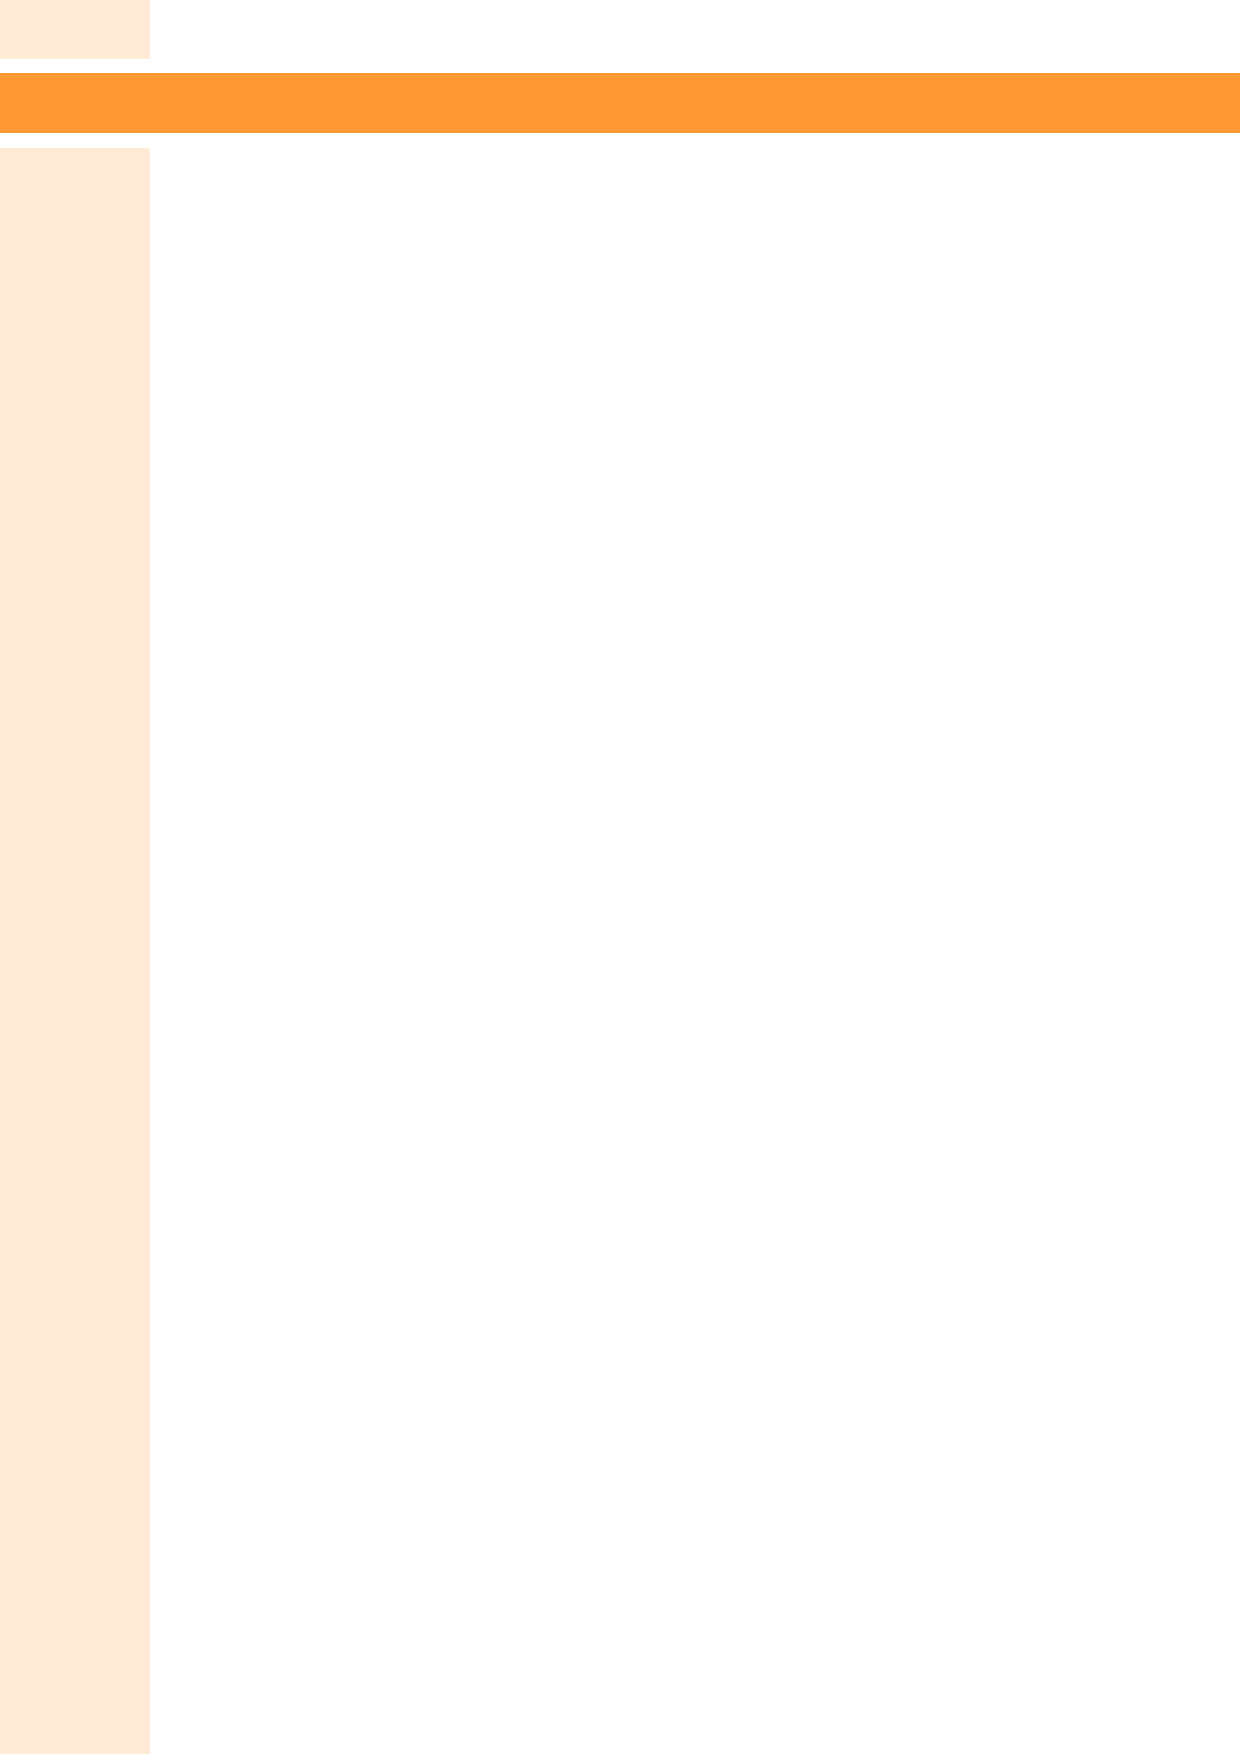
\includegraphics[scale=1]{Cover/cover_background}}}%
  \else
    \ifnum\value{chapter}>0%
      \ifending
        \backgroundsetup{contents={}}%
      \else
        \backgroundsetup{contents={\includegraphics[scale=1]{Cover/chap\thechapter}}}%
      \fi
    \else
    \backgroundsetup{contents={}}%
    \fi
  \fi
}%
{
  \backgroundsetup{contents={}}%
}%
\BgMaterial}
}


% Forcing "squared" paragraph
% ie, the last line is justified.
\newcommand{\startsquarepar}{%
    \par\begingroup \parfillskip 0pt \relax}
\newcommand{\stopsquarepar}{%
    \par\endgroup}
\newcommand{\squarepar}[1]{%
\startsquarepar
#1
\stopsquarepar
}

\usepackage{pifont}
\usepackage{enumitem}
\usepackage{fontawesome}

\newcommand{\inlineitem}{{%
\smaller[1.5]\color{orange}\ding{110}}\hspace{1.5ex}}

\setlist[itemize,1]{%
leftmargin=*,%
itemindent=1em,%
label=\smaller[1.5]\color{orange}\ding{110},%
topsep=0pt,%
itemsep=0pt,%
% partopsep=0pt,%
% parskip=0pt,
}%

\setlist[description]{%
topsep=0pt,%
parsep=4pt,%
labelsep=1em,%
}%

\newlist{features}{description}{1}
\setlist[features]{%
font=\normalfont \em,% first make normal font, then make it emph
% labelwidth=75pt,% (min) size of the description label. Effect: Description text is aligned
% leftmargin=(\labelwidth+\labelsep),%
topsep=0pt,%
parsep=2pt
}

\newlist{subitemize}{itemize}{1}
\setlist[subitemize]{%
leftmargin=*,%
label=\smaller[1.5]\color{orange}\ding{110},%
topsep=0pt,%
itemsep=0pt,%
}

\newlist{functions}{description}{1}
\setlist[functions]{%
font=\normalfont \ttfamily,% first make normal font, then make it tt
topsep=0pt,%
}

% -------------------------------------------------------------------------------------------------
\usepackage{mdframed}
% Definition of new framed environments

% \global\mdfdefinestyle{exampledefault}{%
%   % backgroundcolor=recapbackcolour,
%   backgroundcolor=orange,
% %
%   roundcorner=3pt,
% %
%   % linecolor=black,
%   linewidth=0pt,
%   % topline=true,
%   % rightline=true,
%   % leftline=true,
%   % bottomline=true,
% %
%   shadow=true,
%   shadowcolor=recapshadowcolour,
%   shadowsize=1pt,
% %
%   innertopmargin=5pt,
%   innerbottommargin=5pt,
%   innerleftmargin=5pt,
%   innerrightmargin=5pt,
% %
%   % frametitlerule=false,
%   % frametitlerulewidth=1pt,
%   % frametitleaboveskip=-5pt,
%   % frametitlebelowskip=0pt
% %
%   userdefinedwidth=1.1\linewidth,%
%   leftmargin=-50pt,
% }

\global\mdfdefinestyle{lightgrey}{%,
  backgroundcolor=lightgrey,
%
  roundcorner=3pt,
%
  linewidth=0pt,
%
  shadow=true,
  shadowcolor=midgrey,
  shadowsize=1pt,
%
  % innertopmargin=5pt,
  % innerbottommargin=5pt,
  % innerleftmargin=5pt,
  % innerrightmargin=5pt,
%
  % userdefinedwidth=1.1\linewidth,%
  % leftmargin=-50pt,
}

\global\mdfdefinestyle{lightorange}{%,
  backgroundcolor=lightorange,
%
  roundcorner=3pt,
%
  linewidth=0pt,
%
  shadow=true,
  shadowcolor=midgrey,
  shadowsize=1pt,
%
  innertopmargin=15pt,
  innerbottommargin=15pt,
  innerleftmargin=15pt,
  innerrightmargin=15pt,
%
}

\newenvironment{research_questions}
{
    \begin{mdframed}[style=lightorange]
    \setlist[description]{%
    topsep=0pt,%
    parsep=4pt,%
    labelsep=1em,%
    }%
    {\bf Key Research Questions}
}
{
    \end{mdframed}
}

\newenvironment{publi}
{
    \begin{mdframed}[style=lightgrey]
    \smaller
}
{
    \end{mdframed}
}



% de­fines the boxed­mini­page en­vi­ron­ment — like mini­page, but with a frame around it
\usepackage{boxedminipage}

\usepackage{color,colortbl}
\usepackage{booktabs}

\usepackage{amsmath,amssymb,amsthm}
\usepackage{mathtools}
\makeatletter
\newcommand{\ssymbol}[1]{$^{\@fnsymbol{#1}}$}
\makeatother

\renewcommand{\qedsymbol}{\mbox{\rule[0pt]{1.3ex}{1.3ex}}}

\newcommand{\cvbox}{\mbox{\color{lightorange}\rule[0pt]{\widthof{2012--2013}}{1.5ex}}}



\theoremstyle{plain}
\newtheorem{theorem}{Theorem}
\newtheorem{lemma}{Lemma}
\newtheorem{corollary}{Corollary}

\theoremstyle{definition}
\newtheorem{definition}{Definition}
\newtheorem{example}{Example}
\newtheorem{hypothesis}{Hypothesis}

\theoremstyle{remark}
\newtheorem{remark}{Remark}

\usepackage{graphicx}
\graphicspath{{./Figures/}
{./Figures/Icons/}
{./20_TriScale/Figures/}{./20_TriScale/}
{./30_Baloo/Figures/}
{./40_DRP/Figures/}
{./50_TTW/Figures/}}%helpful if your graphic files are in another directory
\DeclareGraphicsExtensions{.pdf,.jpeg,.png,.jpg}
% Define the size threshold above which a float gets its own page
\renewcommand{\floatpagefraction}{0.8}%

\usepackage[american]{babel}
\addto\captionsamerican{% Replace "english" with the language you use
  \renewcommand{\contentsname}%
    {Table of Contents}%
}

% One may flush out all the un­pro­cessed floats by is­su­ing a \clearpage com­mand, but this has the ef­fect of mak­ing the cur­rent page end pre­ma­turely. Now you can is­sue \af­ter­page{\clearpage} and the cur­rent page will be filled up with text as usual, but then the \clearpage com­mand will flush out all the floats be­fore the next text page be­gins.
\usepackage{afterpage}

% Let you resize text based on its current size (no matter what that may be)
\usepackage{relsize}

% % TikZ stuff
% \usepackage{tikz}
% \usetikzlibrary{patterns}
% \usepackage{scalefnt}
% \usepackage{pgfplots}
% \usepackage{pgfplotstable}
% \usetikzlibrary{shapes}
% \usepackage{tikzscale}

% Pro­vides var­i­ous ways of for­mat­ting the ti­tles of ap­pen­dices
\usepackage{appendix}

% Pro­vides con­trol over the ty­pog­ra­phy of the Ta­ble of Con­tents, List of Fig­ures and List of Tables, and the abil­ity to cre­ate new ‘List of ...’. The ToC \parskip may be changed.
\usepackage[subfigure]{tocloft}

% slimmer formatting and margin, that looks nice(r) for a dissertation
\usepackage{diss}

%% Font stuff
\usepackage{lmodern}
% Renew fonts
\renewcommand{\familydefault}{\sfdefault}

\usepackage[utf8]{inputenc}
\usepackage[T1]{fontenc}

%% Algorithm commands
\usepackage{algorithm}
\usepackage{algorithmicx}
\usepackage{algpseudocode}
\renewcommand{\algorithmicrequire}{\textbf{Input:}}
\renewcommand{\algorithmicensure}{\textbf{Output:}}
\renewcommand{\algorithmiccomment}[1]{{\%#1}}
\DeclarePairedDelimiter{\ceil}{\lceil}{\rceil}
\DeclarePairedDelimiter{\floor}{\lfloor}{\rfloor}

\DeclareMathOperator*{\argmax}{argmax}
\DeclareMathOperator*{\argmin}{argmin}

%% Listing commands
\usepackage{listings}

\usepackage[numbered,framed]{matlab-prettifier}
\lstset{
  style              = Matlab-editor,
  basicstyle         = \mlttfamily,
  escapechar         = ",
  mlshowsectionrules = true,
}



\usepackage[hyphens]{url}
%% PDF metadata
\usepackage[pdftitle={\titlestringNOBR},pdfauthor={Romain Jacob},pdfsubject={Doctoral Dissertation},pdfkeywords={synchronous transmissions, low-power communication, wireless, cyber-physical systems}]{hyperref}
\hypersetup{
  colorlinks=true,
  linkcolor=darkorange,
  urlcolor=darkblue,
  citecolor=darkorange
}

%% References
\usepackage[capitalise, noabbrev]{cleveref}
\crefname{algorithm}{Algorithm}{Algorithms}
\crefname{example}{Example}{Examples}
\crefname{theorem}{Theorem}{Theorems}
\crefname{hypothesis}{Hypothesis}{Hypotheses}
\renewcommand{\chapterautorefname}{Chapter}
\renewcommand{\sectionautorefname}{Section}
\renewcommand{\subsectionautorefname}{Section}
\renewcommand{\subsubsectionautorefname}{Section}
\newcommand{\lemmaautorefname}{Lemma}
\newcommand\figref[1]{\cref{#1}}
\newcommand\Figref[1]{\cref{#1}}
\newcommand\tabref[1]{\cref{#1}}
\newcommand\secref[1]{\cref{#1}}
\newcommand\Secref[1]{\cref{#1}}
\newcommand\chref[1]{\cref{#1}}
\newcommand\algoref[1]{\cref{#1}}
\newcommand\lstref[1]{\cref{#1}}
\def\eqnref#1{Eq.~(\ref{#1})}
\def\Eqnref#1{Eq.~(\ref{#1})}

%% Subfigure and caption formatting
% http://www.peteryu.ca/tutorials/publishing/latex_captions
\usepackage{subcaption}
% \captionsetup{font=small,labelfont={bf,sf}}
\DeclareCaptionFont{tiny}{\tiny}
% \captionsetup{font+=tiny}
% \captionsetup[sub]{font+=tiny}
% \captionsetup[figure]{font=small,labelfont=it,textfont={bf,it}}
%\captionsetup[subfigure]{labelfont=bf,textfont=normalfont,singlelinecheck=off,justification=raggedright}
\captionsetup[figure]{size=small, labelfont=bf, labelsep=quad}
\captionsetup[table]{size=small, labelfont=bf, labelsep=quad}
\captionsetup[subfigure]{size=footnotesize}


\newcommand{\ChapPath}{}
\newcommand{\TablePath}{}
\newcommand{\PathFig}{}
\newcommand{\PathTab}{}

%% Custom command
\newcommand{\fakepar}[1]{\vspace{1mm}\noindent\textbf{#1.}}
\newcommand{\fakeparQM}[1]{\vspace{1mm}\noindent\textbf{#1?}}
\newcommand{\faketitle}[1]{\vspace{2mm}\noindent\textbf{\boldmath#1}}
\newcommand{\etal}{et~al.\xspace}
\newcommand{\eg}{\emph{e.g.},\xspace}
\newcommand{\Eg}{\emph{E.g.},\xspace}
\newcommand{\ie}{\emph{i.e.},\xspace}
\newcommand{\cad}{\emph{\mbox{c.-à-d.}}\xspace}
\newcommand{\etc}{etc.\xspace}
\newcommand{\capt}[1]{\mdseries{\emph{#1}}}
\newcommand{\chal}[1]{\textbf{C#1}}
\newcommand{\question}[1]{\textbf{Question~#1}}
\newcommand{\feature}[1]{\textsl{#1}}

%% Reviews, comments, etc
%\newcommand{\review}[1]{#1}
\newcommand{\review}[1]{{\color{red}#1}}
\newcommand{\red}[1]{{\textcolor{red}{#1}}}
\newcommand{\TODO}[1]{ } % uncomment to skip all todo notes
% \newcommand{\TODO}[1]{\noindent\textit{ \color{red}\textbf{TODO:}~#1} } %LS
\newcommand{\DISCUSS}[1]{\noindent\fbox{\parbox{\linewidth}{ \textit{ \color{blue}\textbf{Discuss:}~#1} }} }

%% chapter-based numbering
\numberwithin{figure}{chapter}
\numberwithin{table}{chapter}
\numberwithin{theorem}{chapter}
\numberwithin{lemma}{chapter}
\numberwithin{example}{chapter}
\numberwithin{definition}{chapter}

%% for subfigures to show chapter number with cref
\makeatletter
\renewcommand\p@subfigure{\thefigure}
\makeatother

%% Protocols/Things names
\newcommand{\baloo}{\textsl{Baloo}\xspace}
\newcommand{\triscale}{\textsl{TriScale}\xspace}
\newcommand{\DRP}{\textsl{DRP}\xspace}
\newcommand{\DRPLong}{Distributed Real-time Protocol\xspace}
\newcommand{\bolt}{\textsl{Bolt}\xspace}
\newcommand{\DPP}{\textsl{DPP}\xspace}
\newcommand{\DPPtwo}{\textsl{DPP2}\xspace}
\newcommand{\blink}{Blink\xspace}
\newcommand{\TTW}{\textsl{TTW}\xspace}
\newcommand{\TTnet}{\textsl{TTnet}\xspace}

%% Short-hand notations
\newcommand{\cps}{CPS\xspace}
\newcommand{\CPS}{CPS\xspace}
\newcommand{\ST}{\text{ST}\xspace}
\newcommand{\iid}{\textsl{i.i.d.}\xspace}

\newcommand{\custommini}[1]{%
\hfill
\begin{minipage}[t]{0.8\linewidth}%
  \setlist[itemize,1]{%
  leftmargin=*,%
  itemindent=1em,%
  label=\smaller[1.5]\color{orange}\ding{110},%
  topsep=0pt,%
  itemsep=0pt,%
  }%
#1\vspace{2pt}
\end{minipage}}

\newcommand{\creditItem}[3]{%
\begin{minipage}[t]{0.12\linewidth}%
  \centering
  \vspace{0pt}
  \includegraphics[height=1.2cm]{#1}
\end{minipage}%
\hfill
\begin{minipage}[t]{0.8\linewidth}%
  ~\\
  #2\\
  used in \cref{#3}
\end{minipage}}

\newcommand{\inlineRef}[3]{%
\emph{#1}\\
#2\\
#3}

\newcommand{\customLink}[4]{%
\makebox[10pt][c]{\larger{\color{orange}#1}}
\hspace{5pt}
\makebox[125pt][l]{#2}
\href{#4}{#3}\\}

\newcommand{\customBox}[1]{%
\makebox[30pt][l]{#1}}

\newcommand{\smallBox}[1]{%
\makebox[20pt][l]{#1}}

\newcommand{\credit}{CRediT\xspace}
\newcommand{\tex}{\TeX\xspace}

% =======================
% All DRP-related symbols
\newcommand{\D}{\mathbf{D}\xspace}
\newcommand{\Dhat}{\widehat{\mathbf{D}}\xspace}
\newcommand{\tfdmin}{\ensuremath{T^{d}_{f, \,min}}\xspace}
\newcommand{\nslotsmax}{\ensuremath{B_{\mathit{max}}}\xspace}
\newcommand{\nodeset}{\ensuremath{\mathcal{N}}\xspace}
\newcommand{\flowset}{\ensuremath{\mathcal{F}}\xspace}
\newcommand{\flow}[1]{\ensuremath{F_{#1}}\xspace}
\newcommand{\flowi}{\flow{i}}
\newcommand{\flowj}{\flow{j}}
\newcommand{\flowany}{\flow{}}
\newcommand{\jitter}[1]{\ensuremath{J_{#1}}\xspace}
\newcommand{\jitteri}{\jitter{i}}
\newcommand{\jitterj}{\jitter{j}}
\newcommand{\jitterany}{\jitter{}}
\newcommand{\flowsrc}[1]{\ensuremath{\mathit{n^s_{#1}}}\xspace}
\newcommand{\flowsrci}{\flowsrc{i}}
\newcommand{\flowdst}[1]{\ensuremath{\mathit{n^d_{#1}}}\xspace}
\newcommand{\flowdsti}{\flowdst{i}}
\newcommand{\flowdstj}{\flowdst{j}}
\newcommand{\latency}[1]{\ensuremath{R_{\mathit{#1}}}\xspace}
\newcommand{\latencyi}{\latency{i}}
\newcommand{\period}[1]{\ensuremath{T_{\mathit{#1}}}\xspace}
\newcommand{\periodi}{\period{i}}
\newcommand{\periodany}{\period{}}
\newcommand{\deadline}[1]{\ensuremath{\mathbf{D}_{\mathit{#1}}}\xspace}
\newcommand{\deadlinei}{\deadline{i}}
\newcommand{\deadlinej}{\deadline{j}}
\newcommand{\deadlineany}{\deadline{}}
\newcommand{\ndeadline}[1]{\ensuremath{D_{\mathit{#1}}}\xspace}
\newcommand{\ndeadlinei}{\ndeadline{i}}
\newcommand{\ndeadlineany}{\ndeadline{}}
\newcommand{\ap}{\ensuremath{\mathit{AP}}\xspace}
\newcommand{\AP}{\ensuremath{\mathit{AP}}\xspace}
\newcommand{\cp}{\ensuremath{\mathit{CP}}\xspace}
\newcommand{\CP}{\ensuremath{\mathit{CP}}\xspace}
\newcommand{\APs}{\ensuremath{\mathit{AP}}s\xspace}
\newcommand{\CPs}{\ensuremath{\mathit{CP}}s\xspace}
\newcommand{\apsrc}{\ensuremath{\mathit{AP_{s}}}\xspace}
\newcommand{\apdst}{\ensuremath{\mathit{AP_{d}}}\xspace}
\newcommand{\cpsrc}{\ensuremath{\mathit{CP_{s}}}\xspace}
\newcommand{\cpdst}{\ensuremath{\mathit{CP_{d}}}\xspace}
\newcommand{\umax}{\ensuremath{\mathit{U_{max}}}\xspace}
\newcommand{\rlength}{\ensuremath{\mathit{C_{net}}}\xspace}
\newcommand{\rperiod}{\ensuremath{\mathit{T_{net}}}\xspace}
\newcommand{\rperiodmin}{\ensuremath{\mathit{T_{net}^{min}}}\xspace}
\newcommand{\rperiodmax}{\ensuremath{\mathit{T_{net}^{max}}}\xspace}

\newcommand{\opwrite}{\textup{\texttt{\small{write}}}\xspace}
\newcommand{\opread}{\textup{\texttt{\small{read}}}\xspace}
\newcommand{\opflush}{\textup{\texttt{\small{flush}}}\xspace}
% =======================



% =======================
% All TTW-related symbols
\newcommand{\appset}{\ensuremath{\mathcal{A}}\xspace}
\newcommand{\persappset}{\ensuremath{\mathcal{A}_{P}}\xspace}
\newcommand{\taskset}{\ensuremath{\mathcal{T}}\xspace}
\newcommand{\messageset}{\ensuremath{\mathcal{M}}\xspace}
\newcommand{\modeset}{\ensuremath{\mathcal{O}}\xspace}
\newcommand{\predG}{\ensuremath{\mathbb{P}}\xspace}
\newcommand{\beacon}{\ensuremath{b}\xspace}

\newcommand{\sched}[1]{\ensuremath{Sched(#1)}\xspace}

\newcommand{\objective}[1]{{\bf(O{#1})\xspace}}
\newcommand{\objA}{\objective{1}\xspace}
\newcommand{\objB}{\objective{2}\xspace}
\newcommand{\constraint}[1]{{\bf(C{#1})\xspace}}

\newcommand{\appl}[1]{\ensuremath{\mathit{a_{#1}}}\xspace}
\newcommand{\appi}{\appl{i}}
\newcommand{\appj}{\appl{j}}
\newcommand{\app}{\appl{}}
\newcommand{\appA}{\ensuremath{\mathit{A}}\xspace}
\newcommand{\appB}{\ensuremath{\mathit{B}}\xspace}
\newcommand{\appX}{\ensuremath{\mathit{X}}\xspace}


\newcommand{\knownApp}[1]{\ensuremath{\mathit{K_{#1}}}\xspace}
\newcommand{\knownAppi}{\knownApp{i}}
\newcommand{\freeApp}[1]{\ensuremath{\mathit{F_{#1}}}\xspace}
\newcommand{\freeAppi}{\freeApp{i}}
\newcommand{\legApp}[1]{\ensuremath{\mathit{L_{#1}}}\xspace}
\newcommand{\legAppi}{\legApp{i}}
\newcommand{\legAppj}{\legApp{j}}
\newcommand{\virtlegApp}[1]{\ensuremath{\mathit{VL_{#1}}}\xspace}
\newcommand{\virtlegAppi}{\virtlegApp{i}}

\newcommand{\minminvirtlegApp}[2]{\ensuremath{\widehat{\virtlegApp{#1}^{#2}}}\xspace}
\newcommand{\minvirtlegApp}[2]{\ensuremath{\widetilde{\virtlegApp{#1}^{#2}}}\xspace}
\newcommand{\minvirtlegAppi}{\ensuremath{\widetilde{\virtlegApp{i}{}}}\xspace}

\newcommand{\cf}[1]{\ensuremath{\mathit{CF({#1})}}\xspace}

\newcommand{\mode}[1]{\ensuremath{\mathit{M_{#1}}}\xspace}
\newcommand{\modeany}{\mode{}}
\newcommand{\modei}{\mode{i}}
\newcommand{\modej}{\mode{j}}
\newcommand{\modeGraph}{\ensuremath{\mathbb{M}}\xspace}
\newcommand{\modeGraphA}{\ensuremath{\mathbb{G}_A}\xspace}
\newcommand{\modeHyperperiod}{\ensuremath{\mathit{LCM}}\xspace}

\newcommand{\Tround}{\ensuremath{T_{r}}\xspace}
\newcommand{\Troundj}{\ensuremath{T_{r_j}}\xspace}
\newcommand{\Troundk}{\ensuremath{T_{r_k}}\xspace}
\newcommand{\Troundmin}{\ensuremath{T_{r}^{\mathit{min}}}\xspace}
\newcommand{\Toffset}{\ensuremath{T_{o}}\xspace}
\newcommand{\Troundon}{\ensuremath{T_{r}^{\mathit{on}}}\xspace}
\newcommand{\Tworound}{\ensuremath{T_{\mathit{wo/r}}}\xspace}
\newcommand{\Tworoundon}{\ensuremath{T_{\mathit{wo/r}}^{\mathit{on}}}\xspace}

\newcommand{\Tslot}{\ensuremath{T_{\mathit{slot}}}\xspace}
\newcommand{\Twakeup}{\ensuremath{T_{\mathit{wake-up}}}\xspace}
\newcommand{\Tstart}{\ensuremath{T_{\mathit{start}}}\xspace}
\newcommand{\Tglossy}{\ensuremath{T_{\mathit{flood}}}\xspace}
\newcommand{\Tflood}{\ensuremath{T_{\mathit{flood}}}\xspace}
\newcommand{\Thop}{\ensuremath{T_{\mathit{hop}}}\xspace}
\newcommand{\Td}{\ensuremath{T_{d}}\xspace}
\newcommand{\Tcal}{\ensuremath{T_{\mathit{cal}}}\xspace}
\newcommand{\Lcal}{\ensuremath{L_{\mathit{cal}}}\xspace}
\newcommand{\Theader}{\ensuremath{T_{\mathit{header}}}\xspace}
\newcommand{\Lheader}{\ensuremath{L_{\mathit{header}}}\xspace}
\newcommand{\Tpayload}{\ensuremath{T_{\mathit{payload}}}\xspace}
\newcommand{\Rbit}{\ensuremath{R_{\mathit{bit}}}\xspace}
\newcommand{\Tgap}{\ensuremath{T_{\mathit{gap}}}\xspace}
\newcommand{\Tpreprocess}{\ensuremath{T_{\mathit{preprocess}}}\xspace}
\newcommand{\Ton}{\ensuremath{T^{\mathit{on}}}\xspace}
\newcommand{\Toff}{\ensuremath{T^{\mathit{off}}}\xspace}
\newcommand{\Lbeacon}{\ensuremath{L_{\mathit{beacon}}}\xspace}
\newcommand{\Lmax}{\ensuremath{L_{\mathit{max}}}\xspace}
\newcommand{\nslotsround}{\ensuremath{B_r}\xspace}
\newcommand{\nslots}{\ensuremath{B}\xspace}

\renewcommand{\prec}{\ensuremath{\mathit{prec}}\xspace}
\newcommand{\map}{\ensuremath{\mathit{map}}\xspace}
\newcommand{\prio}{\ensuremath{\mathit{prio}}\xspace}

\newcommand{\Sij}{\ensuremath{S_{i\setminus j}}\xspace}
\newcommand{\dij}{\ensuremath{d_{ij}^{max}}\xspace}
\newcommand{\Dij}{\ensuremath{D_{ij}}\xspace}
\newcommand{\RTAij}{\ensuremath{rt^{\app}_{ij}}\xspace}
\newcommand{\tiend}{\ensuremath{t^{i}_{end}}\xspace}
\newcommand{\tjstart}{\ensuremath{t^{j}_{start}}\xspace}

\newcommand{\af}{\ensuremath{\mathit{af}}\xspace}
\newcommand{\df}{\ensuremath{\mathit{df}}\xspace}
\renewcommand{\sf}{\ensuremath{\mathit{sf}}\xspace}
\newcommand{\id}{\ensuremath{\mathit{id}}\xspace}
\newcommand{\ids}{\ensuremath{\mathit{id}}s\xspace}
\newcommand{\TB}{\ensuremath{\mathit{TB}}\xspace}
\newcommand{\first}{\ensuremath{\mathit{first}}\xspace}
\newcommand{\last}{\ensuremath{\mathit{last}}\xspace}
\newcommand{\obj}{\ensuremath{\mathit{obj}}\xspace}

\newcommand{\NbOutputn}{\ensuremath{NbOutput(n)}\xspace}
\newcommand{\NbInputn}{\ensuremath{NbInput(n)}\xspace}
\newcommand{\delayOutput}{\ensuremath{T_{r,out}}\xspace}
\newcommand{\delayInputn}{\ensuremath{T_{r,in}(n)}\xspace}
% =======================

% Units
\newcommand{\meter}{\ensuremath{\,\text{m}}\xspace}
\newcommand{\s}{\ensuremath{\,\text{s}}\xspace}
\newcommand{\ms}{\ensuremath{\,\text{ms}}\xspace}
\newcommand{\us}{\ensuremath{\,\mu\text{s}}\xspace}
\newcommand{\ns}{\ensuremath{\,\text{ns}}\xspace}
\newcommand{\minute}{\ensuremath{\,\text{min}}\xspace}
\newcommand{\hour}{\ensuremath{\,\text{h}}\xspace}
\newcommand{\Hz}{\ensuremath{\,\text{Hz}}\xspace}
\newcommand{\kHz}{\ensuremath{\,\text{kHz}}\xspace}
\newcommand{\MHz}{\ensuremath{\,\text{MHz}}\xspace}
\newcommand{\GHz}{\ensuremath{\,\text{GHz}}\xspace}
\newcommand{\dB}{\ensuremath{\,\text{dB}}\xspace}
\newcommand{\dBm}{\ensuremath{\,\text{dBm}}\xspace}
\newcommand{\ppm}{\ensuremath{\,\text{ppm}}\xspace}
\newcommand{\kbps}{\ensuremath{\,\text{kbps}}\xspace}
\newcommand{\MB}{\ensuremath{\,\text{MB}}\xspace}
\newcommand{\pkts}{\ensuremath{\,\text{pkt}/\text{s}}\xspace}
\newcommand{\percent}{\ensuremath{\,\text{\%}}\xspace}
\newcommand{\bytes}{\ensuremath{~\text{bytes}}\xspace}
\newcommand{\kb}{\ensuremath{~\text{kB}}\xspace}
\newcommand{\kB}{\ensuremath{~\text{kB}}\xspace}
\newcommand{\B}{\ensuremath{~\text{B}}\xspace}
\newcommand{\A}{\ensuremath{\,\text{A}}\xspace}
\newcommand{\nA}{\ensuremath{\,\text{nA}}\xspace}
\newcommand{\mbps}{\ensuremath{\,\text{Mbit/s}}\xspace}
\newcommand{\Mbps}{\ensuremath{~\text{Mbit/s}}\xspace}
\newcommand{\V}{\ensuremath{~\text{V}}\xspace}
\newcommand{\mW}{\ensuremath{\,\text{mW}}\xspace}
\newcommand{\uW}{\ensuremath{\,\mu\text{W}}\xspace}
\newcommand{\mA}{\ensuremath{\,\text{mA}}\xspace}

% Link icons

\newcommand{\IconPaper}{\faFileTextO}
\newcommand{\IconPresentation}{\faDesktop}
\newcommand{\IconVideo}{\faFilm}
\newcommand{\IconPoster}{\faColumns}
\newcommand{\IconThesis}{\faBook}
\newcommand{\IconDataset}{\faTable}
\newcommand{\IconImage}{\faFileImageO}
\newcommand{\IconPlot}{\faAreaChart}
\newcommand{\IconCredit}{\faCopyright}
\newcommand{\IconWebsite}{\faGlobe}
\newcommand{\IconTex}{\faFilesO}
\newcommand{\IconData}{\faChain}
\newcommand{\IconCode}{\faCode}
% \newcommand{\Icon}{\fa}
